\subsection{TORCS}


\usebackgroundtemplate{
\begin{picture}(200,350)
\put(2, 78){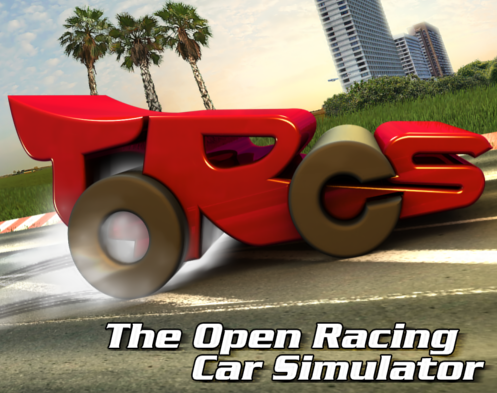
\includegraphics[width=100px]{images/torcs.png}}
\end{picture}
}

\begin{frame}
 \frametitle{TORCS}
 
\begin{center}
  \begin{figure}
      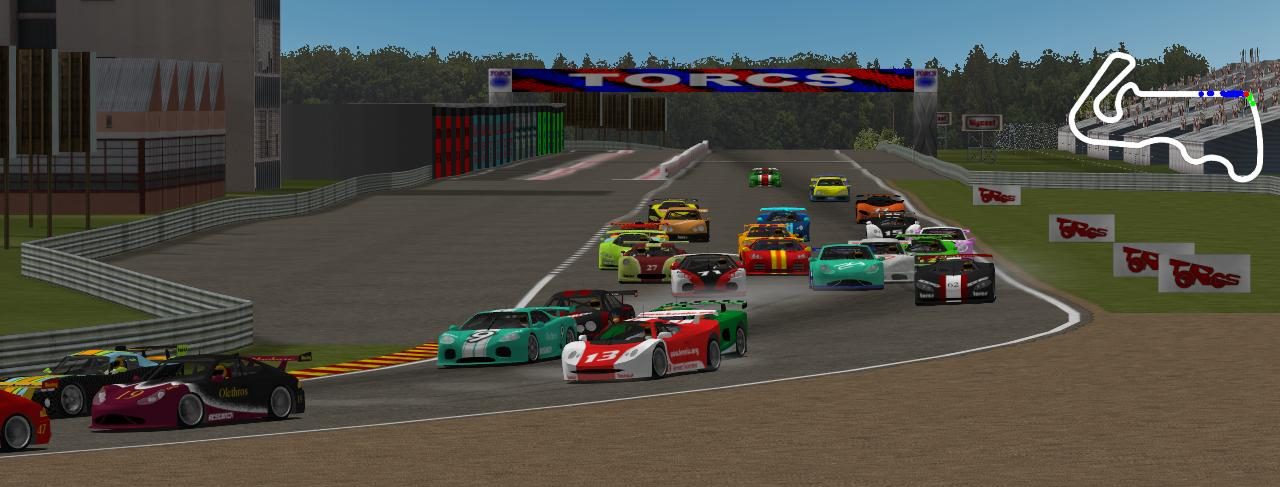
\includegraphics[height=4cm]{images/torcs2.jpg} \\
  \end{figure}
\end{center}
 \vfill
\end{frame}
\usebackgroundtemplate{}

\note{
Le simulateur que nous avons choisi avec nos encadrants est TORCS.

Il permet de simuler des courses de voitures en 3D pour faire
de jolies démos.

Il est open-source et écris en C/C++, très personnalisable,
il permet d'intégrer des modules indépendants pour les agents.

Il permet également d'être simuler sans GUI pour que les agents puissent apprendre.
}

\begin{frame}
 \frametitle{Les entrées}
  
  
  \begin{minipage}{0.5\textwidth}
 \begin{flushleft}
 Capteurs locaux -> généralisation des pistes
 \begin{itemize}
  \item distance au centre 
  \item angle tangent
  \item vitesse
  \item longueur segment
  \item angle prochain virage
 \end{itemize}
  \end{flushleft}
 \end{minipage}
 ~
 \begin{minipage}{0.4\textwidth}
 \begin{flushright}
  \begin{figure}
      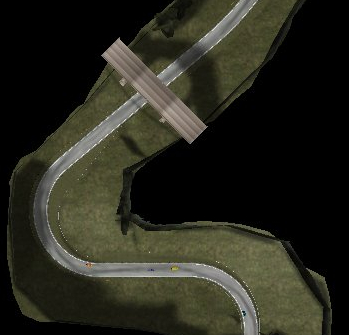
\includegraphics[height=4cm]{images/track.jpg} \\
  \end{figure}
  \end{flushright}
 \end{minipage}

\end{frame}

\note{

[Utiliser l'image]

}

\begin{frame}
 \frametitle{Les actions}

   \begin{minipage}{0.4\textwidth}
 \begin{flushleft}
 \begin{itemize}
  \item Direction
  \item Freinage
  \item Acceleration
  \item Boîte vitesse
 \end{itemize}
  \end{flushleft}
 \end{minipage}
 --- >
 \begin{minipage}{0.4\textwidth}
 \begin{flushright}
 \begin{itemize}
  \item Direction
  \item Vitesse (4 valeurs)
 \end{itemize}
  \end{flushright}
 \end{minipage}
 
\end{frame}

\note{
Dans TORCS il y a en 4 actions possible, qu'on a fusionné en 2 pour simplifier le problème.


Le calcul du changement de boîte à vitesse est automatique.

4 valeurs : acc, ne rien faire,  freiné, reculé.
}

\begin{frame}
 \frametitle{Les récompenses}
  
  
  
\begin{minipage}{0.5\textwidth}
 \begin{flushleft}
Sur route et avance : 
\begin{itemize}
 \item vitesse $\in [100;6000]$
\end{itemize}

Avance pas : - 500 

Avance dans un mur : -1000

Bloqué et Recule : 15

Sens inverse
\begin{itemize}
 \item vitesse $\in [-4000;-2000]$
\end{itemize}

Sort de route 
\begin{itemize}
 \item écart $\in [-1000;-4000]$
\end{itemize}

  \end{flushleft}
 \end{minipage}
 ~
 \begin{minipage}{0.4\textwidth}
 \begin{flushright}
  \begin{figure}
      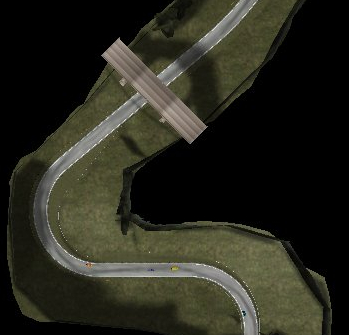
\includegraphics[height=4cm]{images/track.jpg} \\
  \end{figure}
  \end{flushright}
 \end{minipage}
\end{frame}

\note{

}

\begin{frame}
 \frametitle{Demo}

 + Quelques stats

\end{frame}

\note{
L'autre objectif du projet était d'intégrer des feedbacks d'un superviseur à TORCS.
}

\subsection{Feedbacks} 

\begin{frame}
 \frametitle{Mode superviseur}


 Agir sur les récompenses

\end{frame}

\note{
L'autre objectif du projet était d'intégrer des feedbacks d'un superviseur à TORCS.
}

\begin{frame}
 \frametitle{Mode contrôle}

 Agir sur les actions\\
 Montrer à l'agent comment conduire
 Démo

\end{frame}

\note{
Merci aux encadrants, ...
}

